\chapter{Background}

\section{Introduction on ontologies and applications}

\subsection{What is an ontology?}

In artificial intelligence an ontology is 
a formal explicit description of concepts in a domain of discourse properties of each concept describing various features and attributes of the concept, and restrictions on slots. 
The main components of ontologies are classes that represent concepts. Hierarchical relationships exist between classes, meaning a class can have one or more subclasses and super-classes. Additionally, each class is associated with attributes (slots) and restriction rules on the attribute domains (facets). Just as in object-oriented programming, classes are instantiated to create instances that make up the knowledge base.\cite{protege_ontology}
\begin{figure}[H]
    \centering
    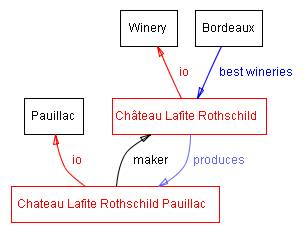
\includegraphics[width=0.5\linewidth]{Figures/fig_0.jpg}
    \caption{Example of a simple ontology in wine domain}
    \label{fig:enter-label}
\end{figure}
\subsection{Classification of ontologies}

Ontologies are useful for representing information in a hierarchical manner (through classes and subclasses), depicting the relationships between the represented information. Based on the level of generality used to describe the present domains, there are four types of ontologies:
\begin{itemize}
    \item \textbf{High-level ontologies:} High-level ontologies describe very general concepts or common-sense knowledge such as space, time, objects, and actions.

    \item \textbf{Domain ontologies:} Domain ontologies describe the vocabulary, theories, and fundamental principles that govern a specific domain.

    \item \textbf{Task ontologies:} Task ontologies describe the vocabulary related to a specific task or activity, providing a specialization of the terms introduced in the high-level ontology.

    \item \textbf{Application ontologies:} Application ontologies describe concepts related to a specific domain or task and are often derived through a specialization of domain ontologies and task ontologies.
\end{itemize}
Ontologies can differ in the way knowledge is expressed, that is, in the level of formalism used to convey terms and their meanings. Therefore, there is an additional classification:
\begin{itemize}
    \item \textbf{Highly informal ontologies:} Highly informal ontologies are expressed in natural language, and the definition of terms may be ambiguous due to the intrinsic ambiguity of natural language.

    \item \textbf{Semi-informal ontologies:} Semi-informal ontologies are expressed in a rigid and structured form of natural language, improving clarity and reducing ambiguities.

    \item \textbf{Semi-formal ontologies:} Semi-formal ontologies are expressed through formally defined artificial languages.

    \item \textbf{Strictly formal ontologies} Strictly formal ontologies are ontologies whose terms are precisely defined with formal semantics, theorems, and property proofs.
\end{itemize}

A further classification can be made based on the expressiveness the ontology aims to convey:
\begin{itemize}
    \item \textbf{Controlled vocabularies:} Controlled vocabularies are finite lists of terms representing the simplest possible notion of an ontology. A typical example is a catalog that provides only terms with an unambiguous interpretation.

    \item \textbf{Glossaries:} Glossaries are lists of terms and their meanings expressed through natural language statements. Primarily created for human use, they often consist of ambiguous statements that cannot be used by automated agents.

    \item \textbf{Thesauri:} Thesauri add semantics to glossaries by defining the relationships between terms (such as synonymy relations). Typically, they do not provide an explicit hierarchical structure, although this can be inferred from the specification of the terms.

    \item \textbf{Informal Is-A hierarchies:} Informal Is-A hierarchies are ontologies in which generalization and specialization are achieved even though there is no strict "sub-class" hierarchy. They include various ontologies available on the Web.

    \item \textbf{Formal Is-A hierarchies:} Formal Is-A hierarchies are ontologies in which concepts are organized according to a strict subclass hierarchy, and the concept of inheritance can always be applied.

    \item \textbf{Frames:} Frames are ontologies in which concepts are described in terms of their characteristic properties. The inclusion of properties in the description of concepts becomes more interesting when inheritance can be applied, allowing properties to be specified for a more general concept and then inherited.

    \item \textbf{Value restrictions:} Value restrictions allow for applying constraints on the values associated with properties.

    \item \textbf{General logical restrictions:} General logical restrictions are usually written in a highly expressive ontological language that allows for the specification of first-order logic constraints on concepts and properties.
    
\end{itemize}
The classifications presented, taken from the Italian study "Ontologie e Linguaggi Ontologici per il Web Semantico" \cite{canfora2004ontologie}, are useful for introducing and better understanding the domains and ways in which ontologies are applied.

\subsection{Applications of ontologies}
Ontologies, therefore, offer the possibility to represent information at various levels in a formal and expressive manner, and for these reasons, they are primarily applied in the following domains: \cite{leonels2023ontology}
\begin{itemize}
    \item \textbf{Information retrieval:} Ontologies can be used to improve the accuracy of search results by helping to understand the meaning of terms and relationships between them.

    \item \textbf{Knowledge management:} Ontologies can help organize and manage knowledge in a more structured and systematic way. They can also facilitate the sharing and reuse of knowledge across different systems and applications.

    \item \textbf{Semantic web:} Ontologies are a key component of the Semantic Web, which aims to make web content machine-readable and understandable by computers.

    \item \textbf{Natural language processing:} Ontologies can be used to improve natural language processing by providing a framework for understanding the meaning of words and sentences.

    \item \textbf{Robotics:} Ontologies can be used to enable robots to better understand their environment and perform tasks more efficiently and accurately.

    \item \textbf{Healthcare:} Ontologies can be used to improve healthcare by providing a standardized way to represent medical knowledge and improve the interoperability of healthcare systems.

    \item \textbf{E-commerce:} Ontologies can be used to improve product search and recommendation systems by providing a more structured and accurate representation of products and their attributes.
\end{itemize}
There are numerous studies and projects in which ontologies and methods for applying ontologies in the mentioned fields have been developed. Regarding information retrieval, the study "The use of ontologies for effective knowledge modelling and information retrieval" \cite{munir2018use} analyzes ontology-based approaches for information retrieval and query formulation on databases. In "Ontology-to-database mapping," a mapping is performed between a relational database and an existing ontology. The mapping is done by representing constructs present in the relational database schema as constructs in the ontology schema and can be achieved using various methods and approaches, including the R2O (Relational to Ontology) language \cite{khan2011r2o}. Another approach described is "Database-to-ontology transformation," where it is assumed that only the relational database exists, and the ontology is created by applying transformation rules. \\
In natural language processing, ontologies can be used to make inferences and to derive rules for semantic interpretation and question-answering systems. In "Natural Language Processing methods and systems for biomedical ontology learning" \cite{liu2011natural} ontologies are applied for the semantic interpretation of clinical documents that is useful to improve questions comprehension and retrieval of correct information.
The use of ontologies in healthcare can be useful for providing information to doctors and patients, improving the quality of medical services. To this end, the study *"Ontology-based Public Healthcare System in Internet of Things"* \cite{kumar2015ontology} describes the implementation of a healthcare information management system based on the Internet of Things. The ontology represents all the concepts and relationships between them necessary to semantically represent the information. The information pertains to healthcare personnel, disease diagnosis, and patient clinical data.\\
As seen in the previously mentioned case, ontologies can be used to represent real-time information, one example of application is robotics. In the paper "OntoSLAM: An Ontology for Representing Location and Simultaneous Mapping Information for Autonomous Robots" \cite{cornejo2021ontoslam} the ontology "OntoSLAM" is created to track in real time all the informations related to robots, those informations are gathered from the robot control system, sensors and actuators. Robots in the environment exchange those informations using a web repository.\\
The presented examples are just a few, but there are thousands of projects where ontologies have been created in a wide range of fields. For this reason, there are online repositories of ontologies, including: \href{https://www.w3.org/wiki/Lists_of_ontologies}{W3.org}, \href{https://archivo.dbpedia.org/list}{DBpedia}, \href{https://agroportal.lirmm.fr/ontologies?search=o}{AgroPortal} and \href{https://bioportal.bioontology.org/ontologies}{BioPortal}. 

\section{Ontology engineering}

\subsection{Competency questions and ontology conceptualization}
The definition of requirements and the subsequent conceptualization are two fundamental steps in ontology design, as they are essential for establishing the objectives, scope of the ontology, and the classes within it. To define the scope and the problems that the ontology should be able to address, designers use competency questions (CQs), which are a set of questions written in natural language that the ontology should be able to answer using its axioms. \cite{malheiros2013method}
In the development of an ontology for noise pollution monitoring \cite{espinoza2020using}, the following competency questions have been defined:

\begin{table}[H]
    \centering
    \begin{tabular}{|>{\raggedright\arraybackslash}p{1cm}|>{\raggedright\arraybackslash}p{6cm}|>{\raggedright\arraybackslash}p{6cm}|}
        \hline
        \textbf{Id} & \textbf{Competency question} & \textbf{Answer} \\ \hline
        \textbf{CQ1} & Which is the measured noise level in a specific moment and location? & The detected noise level during April in location with coordinates 40.42, – 3.69, 648 is 67.4 dB. \\ \hline
        \textbf{CQ2} & Which is the location of a specific measurement station? & The location of the measurement station “Paseo de Recoletos” is 40.42, – 3.69, 648 (Longitude, Latitude, Altitude) \\ \hline
        \textbf{CQ3} & In which day interval the noise level has been detected? & The noise level Ld has been detected in the time interval between 07:00 to 19:00. \\ \hline
        \textbf{CQ4} & Which was the last calibration sensor date? & The datetime, for example, 2017-04-21T14:00:00+01:00 \\ \hline
    \end{tabular}
    \caption{Competency Questions noise pollution ontology}
\end{table}

Each competency question must correspond to a natural language answer that "simulates" the response provided by the ontology. Of course, competency questions are not mandatory for developers but can be used for the creation of methods to translate CQs into ontology queries. An example of a manual translation of a competency question has been done on the African Wildlife Ontology \cite{keet2020african}, where the competency question \textit{"Which plants eat animals?"} was translated into SPARQL-OWL language, resulting in the following code \cite{wisniewski2019analysis}.

\begin{verbatim}
SELECT DISTINCT ?eats
WHERE {
  ?eats rdfs:subClassOf awo:plant, [
    a owl:Restriction ;
    owl:onProperty awo:eats;
    owl:someValuesFrom awo:animal
  ].
  FILTER(?eats != owl:Nothing)
}
\end{verbatim}

The next step, once the competency questions have been defined, is the conceptualization of the ontology, which is useful for defining the classes and the hierarchy among them. There are three approaches to conceptualization:
\begin{enumerate}
    \item \textbf{Top-down:} top-down development process starts with the definition of the most general concepts in the domain and subsequent specialization of the concepts.
    \item \textbf{Bottom-up:}  bottom-up development process starts with the definition of the most specific classes, the leaves of the hierarchy, with subsequent grouping of these classes into more general concepts.
    \item \textbf{Combination:} development process is a combination of the top-down and bottom-up approaches: We define the more salient concepts first and then generalize and specialize them appropriately.
\end{enumerate}
The conceptualization can be carried out by stating classes in a formal system or can be done using diagrams, in this case is important to defined the notation that will be used. 
% vedere se devo aggiungere altro

\subsection{Ontology languages}
Once the requirements have been defined and the classes and entities that make up the ontology have been established, the implementation phase begins. There is a set of languages available for implementing ontologies, with the main standards being RDF (Resource Description Framework) and OWL (Web Ontology Language).\\
RDF is a standard model for data interchange on the Web, it  has features that facilitate data merging even if the underlying schemas differ, and it specifically supports the evolution of schemas over time without requiring all the data consumers to be changed. RDF extends the linking structure of the Web to use URIs to name the relationship between things as well as the two ends of the link (this is usually referred to as a “triple”). Using this simple model, it allows structured and semi-structured data to be mixed, exposed, and shared across different applications.\cite{rdf}\\ 
OWL is a family of knowledge representation for ontologies, the latest version OWL2, born in 2009, is used to build ontologies representing classes, properties, individuals, and data values that are stored as Semantic Web documents.\cite{owl2} % ampliare

\subsection{Ontology engineering methodologies}
The definition of requirements through competency questions and the subsequent conceptualization and implementation fall within the ontology design process, which is studied in ontology engineering. By definition the ontology engineering  is the discipline that investigates the principles, methods and tools for creating and maintaining ontologies. An ontology engineering methodology caters the methodological aspect of ontology development and it gives a set of guidelines and activities to develop ontologies.\cite{iqbal2013analysis}
Over the years, various ontology engineering methods have been proposed; below, I analyze the main methods available in the state of the art.

\subsubsection{METHONTOLOGY}
The first methodology analyzed is \textit{METHONTOLOGY} \cite{fernandez1997ontological} that proposes a structured method which consists of six steps: 
The process begins with the Specification phase, where the goal is to produce an ontology specification document. This document can be informal, semi-formal, or formal, and is written either in natural language or using competency questions to outline the main requirements and scope of the ontology. Next is the Knowledge Acquisition phase, which involves gathering all relevant knowledge related to the domain. This is achieved through various techniques, such as text analysis, brainstorming, interviews, and reviewing existing similar ontologies. The aim is to collect a comprehensive set of information that will serve as the foundation for the ontology. The Conceptualization phase follows, where the acquired knowledge is organized into a conceptual model. This model effectively structures the domain knowledge, describing both the problem and its proposed solution in a coherent manner. During the Integration phase, the methodology encourages reusing and integrating existing ontologies rather than developing new ones from scratch. This step is crucial for ensuring consistency and coherence, as it involves checking libraries of ontologies to find definitions of terms that match the semantics identified in the conceptualization phase. The Implementation phase is where the actual construction of the ontology takes place. Here, the developer selects the appropriate environment and tools to implement the ontology based on the specifications and conceptual model developed in the earlier phases. Finally, the Evaluation phase ensures the quality and correctness of the ontology. This step involves both verification, to confirm that the ontology is technically sound, and validation, to guarantee that the ontology meets the specified requirements. The methodology has the following advantages: 
\begin{itemize}
    \item Methontology identifies all the activities required to develop an ontology, including planning, specification, conceptualisation, formalisation, integration, implementation, evaluation and documentation. 

    \item It proposes the use of an evolutionary prototype life cycle, which allows definitions to be modified, added or removed at any time.

    \item It encourages the reuse of already existing ontologies, which can speed up development and ensure consistency with other projects. 
\end{itemize}
and the following disadvantages:
\begin{itemize}
    \item Methontology is very detailed and rigorous, which can be time and resource consuming, especially for smaller projects, it may be excessive compared to the needs of the project.

    \item The methodology can be complex to master for those without experience in ontology development, as it requires familiarity with several specific techniques and tools.

    \item The methodology has been developed in 1997, making it outdated by today standards. Since its creation, there have been significant advancements in both ontology engineering and related technologies, such as the Semantic Web, Linked Data, and agile methodologies.

    \item The methodology was created before the widespread adoption of agile development practices, which are now a common approach in software and ontology engineering. This makes it less flexible for fast-paced, iterative development environments.
\end{itemize}

\subsubsection{NeOn methodology}
Another proposed methodology is the \textit{NeOn methodology}\cite{neon1}\cite{neon2} which provides guidance for all key aspects of the ontology engineering process. The concepts underlying this methodology are: scenarios, collaborative ontology development, reuse of ontological and non-ontological resources and evolution of networked ontologies. The ontology design is based on nine scenarios:
\begin{enumerate}
    \item \textbf{Scenario 1: From specification to implementation} The ontology network is developed from scratch, developers should specify ontology requirements and search for potential resources to be reused. 

    \item \textbf{Scenario 2: Reusing and re- non-ontological resources}  Developers should carry out the NOR reuse process for deciding, according to the ontology requirements, which NORs can be  reused to build the ontology network. 

    \item \textbf{Scenario 3: Reusing ontological resources} Developers use ontological resources, ontology modules and ontology statements to build ontology networks. 

    \item \textbf{Scenario 4: Reusing and re-engineering ontological resources} Ontology developers reuse and re-engineer ontological resources

    \item \textbf{Scenario 5: Reusing and merging ontological resources} This scenario arises when several ontological resources in the same domain are selected for reuse, and developers wish to create a new ontological resource with the selected resources

    \item \textbf{Scenario 6: Reusing, merging and re- engineering ontological resources} Ontology developers reuse, merge, and re-engineer ontological resources. This scenario is similar to Scenario 5, but here developers decide to re- engineer the set of merged resources

    \item  \textbf{Scenario 7: Reusing ontology design patterns (ODPs)} Ontology developers access repositories to reuse ODPs

    \item \textbf{Scanrio8: Ontology developers access repositories to reuse ODPs} Ontology developers restructure (e.g., modularize, prune, extend, and/or specialize) ontological resources to be  integrated in the ontology network. 

    \item \textbf{Scenario 9: Localizing ontological resources} Ontology developers adapt an ontology to other languages and culture communities, thus obtaining a multilingual ontology.

\end{enumerate}
The scenarios presented are not a rigid workflow, they are more like a variety of pathways for developing ontologies and they  cover commonly occurring situations, for example, when available ontologies need to be re-engineered, aligned, modularized, localized to support different languages and cultures, and integrated with ontology design patterns and non-ontological resources, such as folksonomies or thesauri.\cite{suarez2011neon}\\

The \href{http://neon-project.org/nw/Welcome_to_the_NeOn_Project.html}{Neon project} offers to developers a tool called \href{http://neon-toolkit.org/wiki/Main_Page.html}{NeOn toolkit}: an open-source multi-platform ontology editor which supports the Web Ontology Language OWL2 and features basic editing and visualization functionality.\cite{erdmann2011overview}\\
\begin{figure}[H]
    \centering
    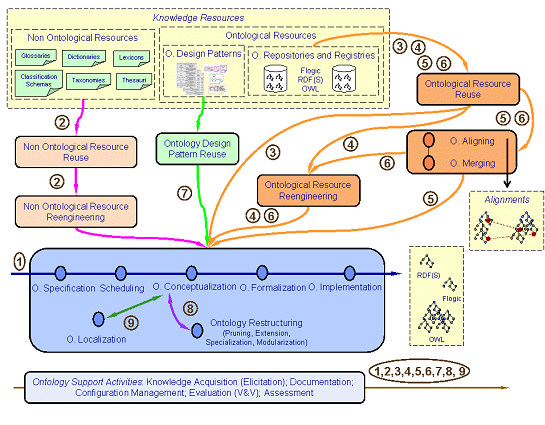
\includegraphics[width=0.5\linewidth]{Figures/fig_2.png}
    \caption{NeOn methodology scenarios}
    \label{fig:enter-label}
\end{figure}
The NeOn methodology has the following advantages:
\begin{itemize}
    \item It identifies nine different scenarios for building ontology networks, which can be combined depending on the project’s needs, this contrasts with more rigid methodologies like METHONTOLOGY.

    \item It supports the reuse and re-engineering of both ontological and non-ontological resources, which can save time and effort by leveraging existing knowledge bases, reducing the need to build everything from scratch.

    \item By basing its structure on real use cases and generalizing from them, the NeOn methodology covers practical needs encountered in ontology development projects.
\end{itemize}
But NeOn has the following disadvantages:
\begin{itemize}
    \item The flexibility and comprehensive nature of the methodology can make it more complex to apply, especially for teams without significant prior experience in ontology development. 

    \item Although NeOn is designed for building large-scale networks, the actual process of merging and aligning different ontologies can be challenging, especially when ontologies come from diverse sources with differing structures and standards.

    \item The methodology is meant to be technology-independent, in practice, it may require specific tools to implement the processes effectively, and these tools might not always be accessible or easy to use for all teams.
\end{itemize}

\subsubsection{Extreme design}
While the NeOn methodology is scenario-based, the eXtreme Design methodology \cite{presutti2009extreme} is based on a sequence of tasks inspired by the principles of agile development in software engineering. eXtreme Design involves the client in order to gather complete requirements without making incorrect assumptions. This interaction is useful for defining competency questions and customer stories that detail the use of the ontology, supported by contextual statements that make implicit knowledge explicit. The principles of eXtreme Design not only focus on the client but also provide clear guidelines to designers regarding the design and organization of work. In particular, the design must be modular and task-oriented, focusing on the specifications defined in the competency questions. These competency questions are used in the development of unit tests during the testing phase, verifying the compliance of the ontology with the user stories. Tests are generally conducted using SPARQL queries that encode the competency questions. Throughout the development phase, the designers are organized according to the \textit{pair design}, where the design team is divided into pairs that must collaborate, sharing knowledge and integrating the various parts of the ontology developed. Based on the principles illustrated, eXtreme design defines adisci task: 
\begin{enumerate}
    \item \textbf{Task 1. Get into the project context:} The development process begins by aligning the designers and domain experts, who may have different backgrounds and terminologies. The goal is twofold: to familiarize the customer with the project's methods and tools, and to provide the designers with an understanding of the problem, scope, and initial terminology, establishing a collaborative environment for sharing documentation and discussing modeling issues.

    \item \textbf{Task 2. Collect requirement stories:} The customer writes stories starting from real scenarios in order to sample the typical facts that should be stored in the ontology.

    \item \textbf{Task 3. Select a story that has not been treated yet:} Each pair of designers selects a story to focus on for the next iteration, creating a new wiki page with the story's title and content based on the information from the card.

    \item \textbf{Task 4. Transform the story into CQs:} Starting from the wiki created in the previous task, designers create a sequence of competency questions, this task involves customer for having feedback/clarifications.

    \item \textbf{Task 5. Select a CQ that has not been treated yet:} The iteration continues by selecting one of the CQs.

    \item \textbf{Task 6. Match the CQ to GUCs:} This task aims to identify candidate Content Patterns (CPs) based on the Competency Questions (CQs) that express part of the Logical Unit of Concern (LUC). Matching can be done with tool support, such as keyword-based searching, or manually by designers familiar with available CPs.

    \item \textbf{Task 7. Select the CPs to reuse:} The goal of this task is to select which of those patterns should be used for solving the modeling problem. 

    \item \textbf{Task 8. Reuse and integrate selected CPs:} . The term “reuse” here refers to the application of typical operation that can be applied to CPs i.e. import, specialization, and composition. 

    \item \textbf{Task 9. Test and fix:} The goal of this task is to validate the module by ensuring it aligns with the Competency Questions (CQs) just modeled. This process involves several steps: first, the CQ is transformed into a unit test, such as a SPARQL query, then, the module is populated with sample data based on the story, and the test is run. If the result isn't as expected, the module is revised and the test is rerun until it passes and once all tests linked to the story have been successfully completed, the designers can move on to the next task. If any CQ remains unaddressed, they return to an earlier task to make adjustments.

    \item \textbf{Task 10. Release module:} This tasks ends the development phase and releases an ontology module having an URI shared with the whole team and on web repositories.

    \item \textbf{Task 11. Integrate, test and fix:} After the module is released it has to be integrated with the other modules that constitute the ontology. 
\end{enumerate}
Once the eleven tasks have been completed, the release of the new version of the ontology takes place. 
The eXtreme design methodology has the following advantages:
\begin{itemize}
    \item The methodology supports collaboration and modular ontology development, allowing teams to work on different parts of the ontology in parallel, which is especially useful for large and distributed projects.

    \item It employs a test-driven approach, where competency questions and contextual statements serve as the basis for unit testing the ontology, ensuring that each component meets its intended purpose before moving forward.

    \item The methodology emphasizes constant interaction with domain experts and stakeholders to ensure that the ontology meets the intended use and requirements. This minimizes assumptions and ensures that implicit knowledge is captured
\end{itemize}
But there are some disadvantages:
\begin{itemize}
    \item The methodology's iterative, test-driven nature may be overkill for smaller ontology projects, where a simpler, more direct approach could be more efficient.

    \item Effective use of XD relies on the availability of supporting tools, such as the NeOn Toolkit and its XD plugin. While these tools are valuable, they may limit accessibility if they are not well-maintained or widely available.
\end{itemize}

\subsection{LOT Methodology}
The \textit{LOT Methodology} (Linked Open Terms) \cite{poveda2022lot} introduces a lightweight industrial-oriented method for developing ontologies. The methodology is compatible with software development techniques, in fact it is inspired by the agile methodology and it defines a basic workflow consisting in four steps:
\begin{figure}[H]
    \centering
    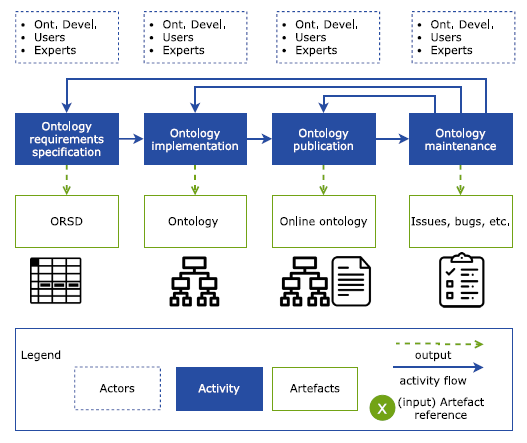
\includegraphics[width=0.5\linewidth]{Figures/fig_3.png}
    \caption{LOT methodology base workflow}
    \label{fig:enter-label}
\end{figure}


\textbf{1 - Ontology requirements specification}\\
In this phase there is the definition of of the domain that the ontology should model, the goal of the ontology and the implementation language. In detail there are seven steps as shown below:
Initially, use case specifications are created in collaboration with domain experts, users, and ontology engineers. These use cases describe scenarios in which the ontology will be utilized, expressed in natural language. Next, data exchange identification is carried out, where the necessary documentation and resources related to the domain are gathered and compiled into a set of documents. This provides a foundation for understanding the context and requirements of the ontology. The purpose and scope of the ontology are then identified with input from users and domain experts. The purpose clarifies the reason for creating the ontology, while the scope defines the aspects of the domain that will be represented. Subsequently, a set of functional ontological requirements is proposed, often in the form of competency questions (CQs) or natural language statements. These requirements outline what the ontology should be able to answer or represent. Ontology experts then review these functional requirements to ensure their correctness and completeness, addressing any ambiguities and verifying consistency with the defined purpose and scope. Following this, the Ontology Requirements Specification Document (ORSD) is formalized. This document consolidates all the information, competency questions, and functional requirements defined in the earlier phases, serving as a comprehensive reference for the ontology development. In some cases, an optional activity is conducted where the functional ontology requirements are further formalized into test cases, expressed in SPARQL queries. This step helps in validating that the ontology meets the specified requirements through structured testing.

\textbf{2 - Ontology implementation}\\
In this phase the ontology is implemented using a formal language, first there is the conceptualization in which there is the definition of classes, sub-classes, relationships and axioms. In the encoding phase there is the actual creation of the ontology using an implementation language, in this phase is useful to take into account other similar ontologies that could be reused. Once the whole ontology is completed it can be evaluated according different evaluation criteria. \\
\textbf{3 - Ontology publication}\\
In this phase the ontology is published online, making it accessible and searchable by users. Before publishing the ontology online, it is necessary to identify the version to be released, document the ontology using human-readable HTML pages, and finally publish the ontology online according to W3C guidelines.\cite{ontology_online}\\


\textbf{4 - Ontology maintenance}\\
The last step is the ontology maintenance, in this phase once the ontology is published online there is bug detection but it also useful in order to update the ontology according new requirements.\\

\textbf{Application of LOT methodology}\\
Despite being introduced recently, the LOT methodology has been successful and has been applied in several projects, both in research and in the industrial field, for the development of ontologies. In the industrial and manufacturing sector, the ontology \textit{SAREF4INMA} \cite{de2020saref4inma} has been developed to describe equipment, materials, products, factories and manufacturing processes in a structured way. The industry is not the only sector where an ontology developed with the LOT method can be applied. In Spain, specifically in Madrid, an ontology has been developed to represent the Bus Public Transport system. \cite{ruckhaus2023applying} The ontology represents information on lines, routes, journey patterns and their timetables, stops on each route, information on expected bus arrival times for each stop, and information on planned and unplanned incidents that may affect the bus routes and their journeys. Still in Spain the LOT methodology has been successfully used in the development of a noise pollution ontology.\cite{espinoza2020using} The ontology integrates data from IoT sensors in the city and establishes semantic relationships between them. The LOT methodology has been used also in artificial intelligence research field, the \textit{HALO ontology} \cite{nananukul2024halo} has been creating for representing hallucinations in large language models. In the ontology there are classes for representing LLMs, hallucinations (with subclasses), prompts and responses. The ontology consists of two modules and was created from a dataset of 40 known prompts designed to generate hallucinations. Each prompt was given as input to three large language models: ChatGPT, BARD, and Claude.
\begin{figure}[H]
    \centering
    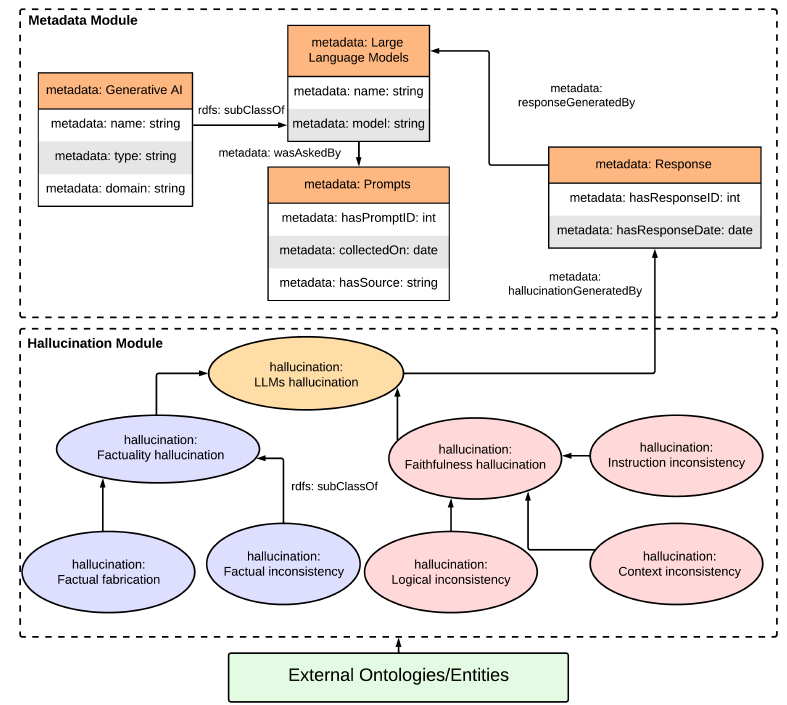
\includegraphics[width=0.7\linewidth, height=8cm]{Figures/fig_4.png}
    \caption{HALO ontology}
    \label{fig:enter-label}
\end{figure}
The LOT methodology has the following advantages:
\begin{itemize}
    \item The LOT methodology is designed to be lightweight and agile, which allows for faster iterations and easier integration with software development practices and it is particularly well-suited for projects that need rapid, iterative development.

    \item The methodology provides a structured approach, including well-defined steps such as ontology requirements specification, implementation, publication, and maintenance.

    \item It offers flexibility by combining various techniques ( competency questions, natural language statements ...) to define requirements and allows for different levels of formality depending on the project.

    \item Many open source ontologies have been developed successfully using LOT methodology for example the HALO ontology, the public transport ontology and may others described previously.
\end{itemize}
but the LOT methodology has two disadvantages:
\begin{itemize}
    \item LOT encourages the reuse of existing ontologies, but this can be challenging due to the potential inconsistencies and heterogeneity of reused ontologies. The methodology does not fully address how to resolve these issues.

    \item The emphasis of LOT on formal validation processes (such as the use of SPARQL queries) may not be sufficient for certain complex domains or non-technical stakeholders.
\end{itemize}

\subsection{Ontology engineering using large language models}
The methodologies analyzed for ontology design involve users, domain experts, and ontology engineers, but do not include the use of advanced tools based on artificial intelligence, such as large language models. The spread of large language models has opened a new path for the design and construction of knowledge graphs and ontologies in an automatic or semi-automatic manner. The study "From human experts to machines: An LLM supported approach to ontology and knowledge graph construction"\cite{kommineni2024human} introduces a semi-automatic pipeline for the construction of knowledge graphs. There are six phases in the proposed pipeline.
The process begins with the data collection phase, which does not involve the use of large language models (LLMs). Instead, domain experts generate a dataset and a set of publications relevant to the topic under study.
In the next phase, known as competency question (CQ) generation, ChatGPT-3.5 is utilized to create competency questions. These questions are designed to describe the data collected in the previous phase at an abstract level. Domain experts provide inputs to the LLM to generate these questions, which are then evaluated by two domain experts to ensure their relevance and accuracy. Following this, the ontology creation phase is initiated. It builds on the competency questions generated earlier. This phase involves two steps: in the first step, a prompt is created that includes a competency question, the expected output, and a set of instructions. In the second step, the LLM is provided with a basic ontology structure containing the concepts and relationships derived from the competency questions.
The CQ answering phase involves applying text processing techniques to extract answers to the competency questions. These answers are used to enrich the ontology and provide a deeper understanding of the dataset.
During the knowledge graph (KG) construction phase, the competency questions, their answers, and the ontology generated by the LLM are combined and provided as input to the LLM. The prompt for this phase focuses on extracting entities, relationships, and concepts and mapping them onto the ontology, thereby creating a comprehensive knowledge graph.
Finally, in the evaluation phase, the LLM evaluates the competency questions and the constructed knowledge graph by comparing them to a ground truth generated by human evaluators. The LLM assigns a score based on the alignment of the generated knowledge graph with the human-generated ground truth.
The presented method enabled the creation of a fairly complex ontology consisting of 45 classes, 41 relations, and 365 axioms. However, it required significant computational resources, as an 80GB NVIDIA A100 GPU machine was used. \\
Another approach for ontology learning using large language models is NeOn-GPT.\cite{fathallah2024neon} Starting from the NeOn methodology, the methodology is converted to a series of prompts to ChatGPT-3.5, these prompt are created using prompt engineering techniques and they are used first to generate ontology specification and competency questions. ChatGPT-3.5 is used also to generate a conceptual model of the ontology in the form of subject-relation-object triples and to generate implementation code. Once the code is generated, there is the syntax validation using the RDFLib python library\cite{rdflib} and the consistency check in order to check logical inconsistencies. The final step is the pitfall resolution for checking circular axioms and missing disjointedness using OOPS API. The presented methodology is an evolution of the NeOn methodology, in which all tasks traditionally performed by the developer are delegated to ChatGPT. This includes identifying requirements, writing competency questions, conceptualizing, and implementing the ontology.\\
ChatGPT can be used not only for the creation of ontologies but also for the creation of more complex knowledge graphs, specifically Hyper-Relational Knowledge Graphs, as discussed in the study "Construction of hyper-relational knowledge graph using pre-trained large language models".\cite{datta2024construction} Hyper-relational knowledge graphs unlike the normal knowledge graphs incorporate additional qualifiers or attribute-value pairs\cite{hyper}, in the study starting from HyperRED dataset, a dataset about different topics , the hyper relational knowledge graph is built including in prompts the data from the dataset. Prompts are generated using Chain-of-Thoughts prompt engineering technique (CoT) and in order to evaluate the result generated, BERTScore is choose as a metric. The results obtained were not satisfactory, as the other algorithm(CubeRE)for extracting hyper-relational information was not surpassed.\\
In general, large language models have shown promising potential  in automating and enhancing the processes of ontology and knowledge graph construction replacing the ontology engineer in different tasks.

\newpage
\section{Large language models}
\subsection{Overview of large language models}
Large language models, as seen in the previous section, are capable of supporting the development of ontologies by ontology engineers, but this revolutionary technology in the field of artificial intelligence is applied to various tasks across diverse domains, thanks to the incredible versatility these models offer. Starting from the definition, a large language model is a large-scale, pre-trained statistical language model based on neural networks, it is capable of language generation and other natural language processing tasks.\cite{llm_wiki} Large language models are trained on a vast amount of training data in order to predict the next word in a given sequence of words, no matter if that sequence is long or short, it can be in any other language and it can include mathematical formulas and even sequences of code.\cite{llm_medium} An important feature that distinguishes large language models from other models is their ability to perform tasks they have not been specifically trained on. In fact, compared to other models, large language models are \textit{zero-shot reasoners}: when given an instruction without any example of the task (zero-shot), they are able to provide a correct response. This has been proved in the study \textit{Large Language Models are Zero-Shot Reasoners} \cite{kojima2022large}, using the prompting technique called \textit{"Zero-shot-CoT"} the study proves the reasoning ability of llms like OPT, GPT, T0 and PaLM on problems divided into four categories: arithmetic, common sense, symbolic and data understanding. On those problems in which llms have to "think step-by-step", they have demonstrated a good accuracy around 70\%.\\
Large language models are able to execute different heterogeneous task tanks to a complex neural-network architecture under the hood, the most advanced architecture is the transformer architecture. Introduced in the 2017 by the study \textit{Attention Is All You Need}\cite{vaswani2017attention} the architecture is composed by two parts:
\begin{enumerate}
    \item \textbf{Encoder:} the encoder has six layers, each layer has a multi-head self-attention mechanism and a position-wise fully connected feed-forward network.

    \item \textbf{Decoder:} the decoder has six layers, it has a sub layer that performs multi-head attention over the encoder’s output. The self-attention mechanism in the decoder is modified to prevent future positions from influencing past positions, ensuring autoregressive property.
\end{enumerate}
The multi-head attention mechanism projects the queries, keys, and values into multiple subspaces, allowing the model to attend to different parts of the sequence simultaneously and in parallel.
\begin{figure}[H]
    \centering
    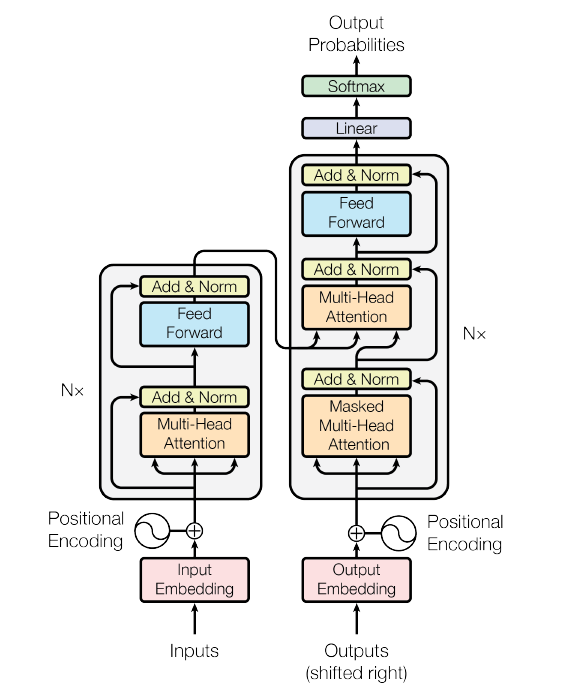
\includegraphics[width=0.5\linewidth]{Figures/fig_17.png}
    \caption{Transformer architecture}
    \label{fig:enter-label}
\end{figure}
The transformer architecture has shown good performances and it is used by one of the most popular llm: GPT-3 \cite{gpt_dugas} but there are other architectures\cite{naveed2023comprehensive}:
\begin{itemize}
    \item \textbf{Encoder-Decoder architecture:} this architecture processes inputs through the encoder and passes the intermediate representation to the decoder to generate the output.\cite{encoder_medium}

    \item \textbf{Casual Decoder architecture:} this architecture does not have an encoder and it uses a decoder in order to generate tokens, each token depends on the previous sequence. \cite{uniteai_decoder}

    \item \textbf{Prefix Decoder architecture:} this architecture is a modification of the causal decoder architecture, it has a bidirectional attention mechanism that can encode the prefix sequence bidirectionally and predict output tokens autoregressively using shared parameters. \cite{llm_labeller}
\end{itemize}
Zero-shot reasoning, made possible by the described architectures, turns large language models into general-purpose tools capable of understanding natural language text and performing tasks ranging from simple text translation to more complex tasks such as question-answering and even code generation. The utility of these models makes them perfect for everyday use, and they find applications in various fields. 

\newpage
\subsection{General purpose large language models}
General purpose large language models are large language models capable of performing a wide variety of tasks and are available online. In this section, I will analyse and discuss the following general purpose large language models.
\begin{itemize}
    \item \textbf{GPT}
    \item \textbf{BERT}

    \item \textbf{PaLM}

    \item \textbf{LLaMA}

    \item \textbf{T5}
    
    \item \textbf{BLOOM}

    \item \textbf{Mistral}
\end{itemize}

\subsubsection{GPT}
The Generative Pretrained Transformer (GPT) is actually the most advanced and powerful large language models available to users. The LLM has been developed by OpenAI and it has been made available to the public in November 2022 in form of a web application called ChatGPT. In two months it gained over than 100 million of users, making it the  fastest-growing consumer software application in history, this massive success it is due to its capacity of understanding user language supporting him in different task.\cite{chatgpt_wiki} 
\begin{figure}[H]
    \centering
    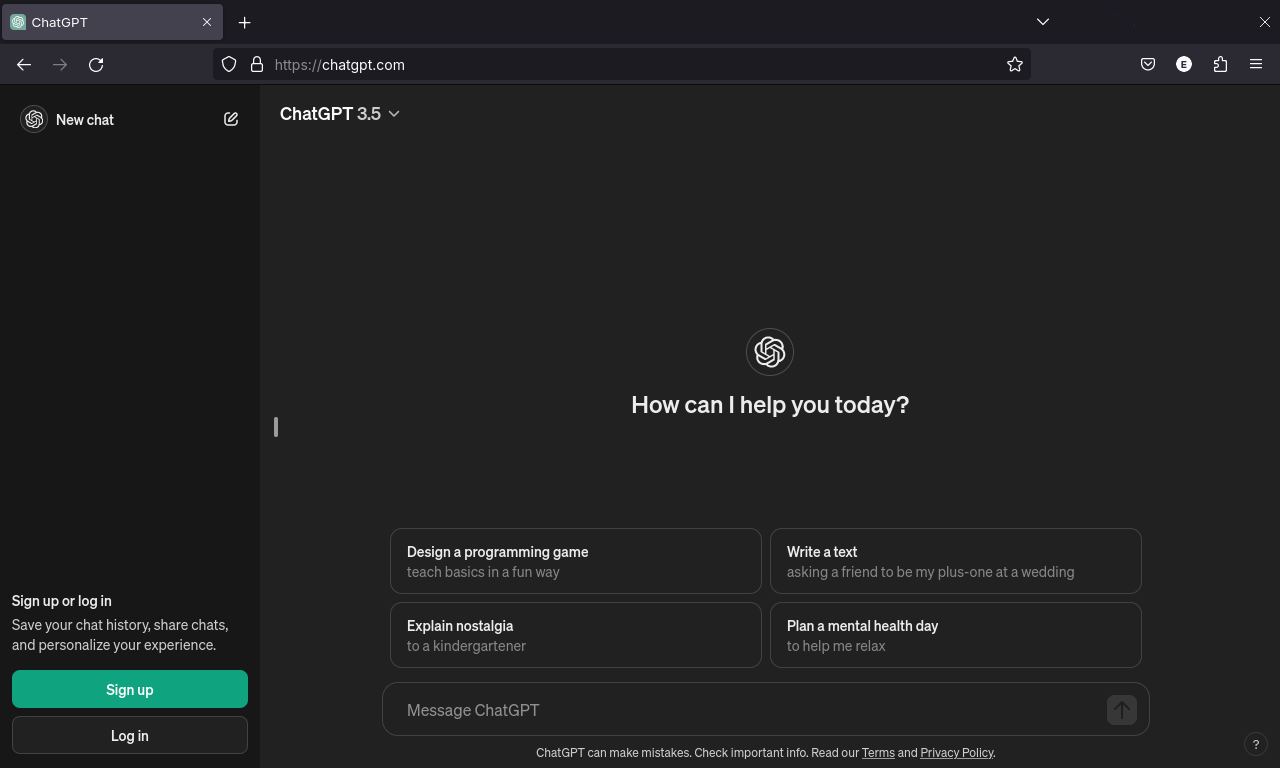
\includegraphics[width=0.9\linewidth]{Figures/fig_18.png}
    \caption{ChatGPT interface}
    \label{fig:enter-label}
\end{figure}
Since its first version, GPT-1 released in 2018, the model represented a step forward in AI development because it was able to comprehend textual material in a more natural manner than before, it had 117 million parameters and it was trained on the BookCorpus dataset. The model was improved in 2019 with the next version: GPT-2 which had 1.5 billions of parameters and it was trained on WebText dataset with 8 millions of documents.\cite{radford2019language} In 2020, OpenAI released GPT-3: this version is more powerful than GPT-2, it is trained over one trillion of internet resources and it has 175 billions of parameters. It is able to perform \textit{in-context learning}, the model recognize pattern in data which is useful when it has few example or just a task description. \cite{journey_gpt}
The latest version of GPT is GPT-4, this large language model is a multimodal model, it can take as input images and text and generate a response. Despite the continuous evolution and the billions of parameters of the model, it is still subject to issues, including hallucinations: it is unable to provide a correct answer and instead outputs false information.\cite{achiam2023gpt}
\subsubsection{BERT}
BERT (Bidirectional Encoder Representations from Transformers) was introduced by Google AI in 2018 and it is described in the paper \textit{"BERT: Pre-training of Deep Bidirectional Transformers for Language Understanding"}.\cite{kenton2019bert} Compared to other models like GPT, BERT is a bidirectional transformer-based model: it takes into account the context on the left and on the right of each word in order to get better understanding of the text. This goal is achieved during the pre-training phase: in the training corpus. tokens are masked randomly allowing the model to predict missing tokens in the text. The pre-training is based on the BookCorpus dataset\cite{bandy2021addressing} and on english Wikipedia. Moreover BERT is able to perform the next sentence prediction nlp task\cite{shi2019next}, predicting a sentence on the basis of the previous sentence.\\
BERT model is used mainly for sentiment analysis and text classification, unlike GPT, it does not have a web interface, but the different versions of BERT are available on Huggingface at this link:\\ https://huggingface.co/docs/transformers/model\_doc/bert.
\subsubsection{PaLM}
In September 2023, Google AI released a more powerful model: PaLM (Pathways Language Model), this model has 540 billions of parameters using a dense decoder-only Transformer model trained with the Pathways system that allows parallel training. \cite{anil2023palm}\cite{barham2022pathways}
PaLM is trained  using a combination of English and multilingual datasets (100 languages) that include high-quality web documents, books, Wikipedia, conversations, and GitHub code, this dataset allows PaLM to do complex reasoning and code generation.\cite{palm2_intro} PaLM is a general purpose large language models but more specialized versions have been developed: 
\begin{itemize}
    \item \textbf{Med-PaLM 2:} this version of PaLM is specifically trained medical text and it is able to give in output medical diagnosis. 
    \item \textbf{Sec-PaLM:} this version of PaLM is applied to cybersecurity, it can analyze and detect malicious scripts that ca be a threat for companies.
\end{itemize}
PaLM represents a significant step forward in large language models and is the direct competitor to GPT. Additionally, it serves as the starting point for an even more powerful multimodal model: Google Gemini, which I will discuss in the following section.
\subsubsection{LLaMA}
LLaMA (Large Language Model Meta AI) is a family of large language models developed by another web giant: META developed introduced in 2023. LLaMA models are based on transformer architecture and, like PaLM, they are trained using different sources, specifically: EnglishCommonCrawl dataset, C4 dataset, Github, Wikipedia, ArXiv and Stack Exchange.  Thanks to the extensive dataset LLaMA models are able to perform common sense reasoning, question-answering, mathematical reasoning, text comprehension and code generation, those abilities have been assessed using zero-shot and few-shot prompting. \cite{touvron2023llama}\\The latest version LLaMA 3 includes over 400 billions of parameters\cite{llama3_intro} and it can be downloaded on huggingface or on the official meta website. More specific LLaMA versions have been developed:
\begin{itemize}
    \item \textbf{Code LLaMA:} Code Llama is a family with the capabilities to accept text prompts and generate and discuss code. The release also includes two other variants (Code Llama Python and Code Llama Instruct) and different sizes.
    \item \textbf{LLaMA Guard:} LLaMA Guard is an LLM-based input-output safeguard model geared towards Human-AI conversation use cases. The model an LLM-based input-output safeguard model geared towards Human-AI conversation use cases.
    \item \textbf{LLaMA 3.2 Vision:} the most advanced version of LLaMA that supports visual prompts.
\end{itemize}
Moreover these version, a version of LLaMA 2 called "LLaMAntino"\cite{basile2023llamantino} that has been created by researchers of the University of Bari ant it is trained on the Italian corpora.
\subsubsection{T5}
T5 (Text-to-Text Transfer Transformer) is an encoder-decoder model, introduced in 2020, pre-trained on a multi-task mixture of unsupervised and supervised tasks\cite{raffel2020exploring} and for which each task is converted into a text-to-text format. The model has been trained on CommonCrawl dataset that includes 750 GB of english text in addition to Wikipedia and RealNews-like dataset.
There are five version of the T5 model:
\begin{enumerate}
    \item \textbf{T5-Base:} 220 millions of parameters.
    \item \textbf{T5-Small:} 60 million of parameters.
    \item \textbf{T5-Large:} 770 million of parameters.
    \item \textbf{T5-3B:} 3 billions of parameters.
    \item \textbf{T5-11B:} 11 billions of parameters.
\end{enumerate}
\begin{figure}[H]
    \centering
    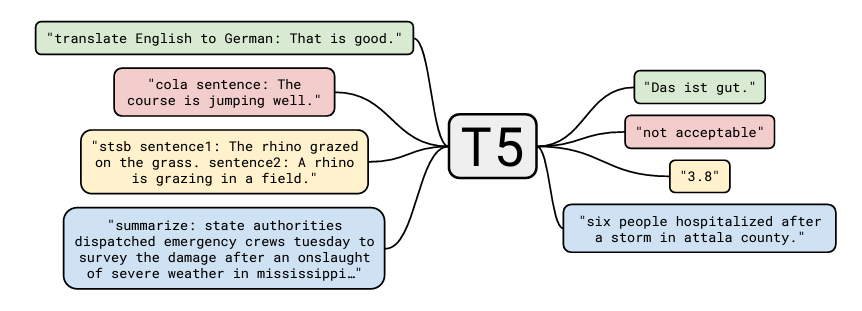
\includegraphics[width=0.8\linewidth]{Figures/fig_19.png}
    \caption{Unified text-to-training}
    \label{fig:enter-label}
\end{figure}
All version of T5 are able to perform different tasks including:\cite{t5_docs}
\begin{itemize}
    \item Text Classification: T5 can classify sentences or documents, it can perform sentiment analysis, grammatical judgments, or assign labels to questions based on their type.

    \item Translation: T5 can translate text between different languages, for example from English to German.

    \item Question Answering: Given a context and a question, the model can provide an accurate answer.

    \item Summarization: T5 can summarize longer documents or articles, generating a brief summary of the content.

    \item Logical Inference: T5 can handle natural language inference tasks where it determines whether one sentence entails, contradicts, or is neutral in relation to another sentence.
\end{itemize}
All the version of T5 models are available on Huggingface at the link:\\
https://huggingface.co/docs/transformers/model\_doc/t5
using the transformers python library.

\subsubsection{BLOOM}
BLOOM (BigScience Large Open-science Open-access Multilingual Language Model) is an open source autoregressive large language model trained to continue text from a prompt on vast amounts of text data using industrial-scale computational resources. In detail the model has 175 billions of parameters and it is trained on a dataset that includes 46 natural languages and 13 programming languages in form of 350 billions of unique tokens.\cite{le2023bloom} BLOOM actually is the biggest and the most powerful open source large language model and it can be used for multilingual content generation, software development and research.\cite{exploring_bloom} The BLOOM llm is available on Huggingface at the link: https://huggingface.co/bigscience/bloom using the transformers python library.
\subsubsection{Mistral}
Mistral is a seven-billion parameters large language models released in September 2023 by the french startup Mistral-AI, the model, like others analyzed, is based on the transformer architecture and it has free versions and premium version available.\cite{jiang2023mistral} Mistral has text and code generation capabilities and it can be used using a web interface available at the link: https://chat.mistral.ai/chat. 
\begin{figure}[H]
    \centering
    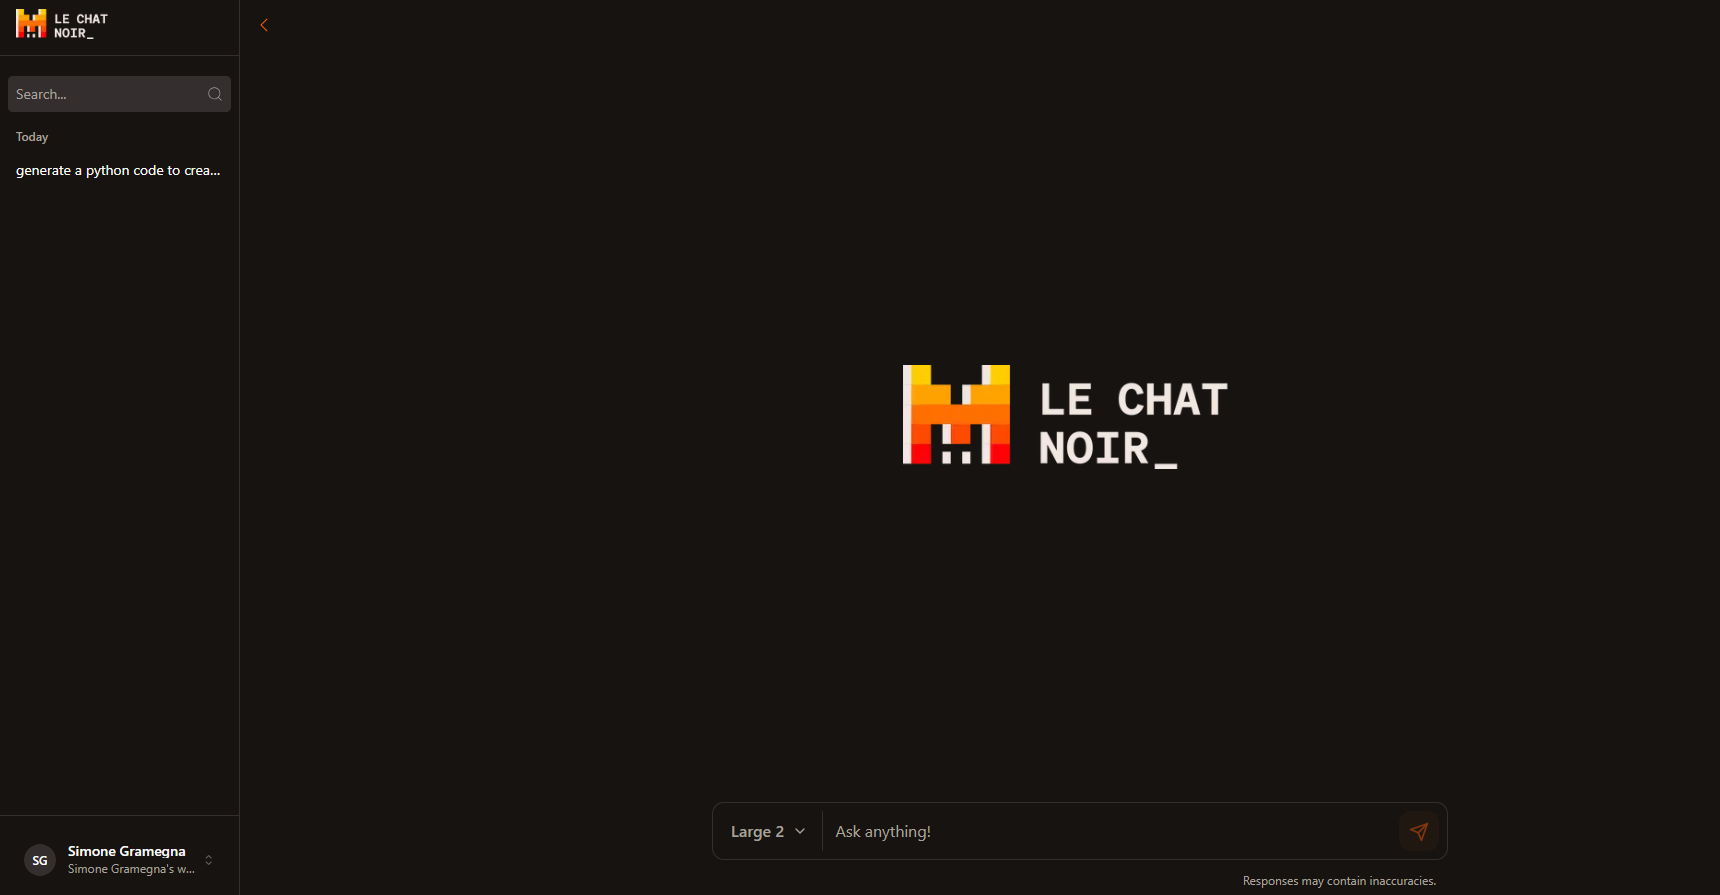
\includegraphics[width=0.9\linewidth]{Figures/fig_20.png}
    \caption{Mistral web interface}
    \label{fig:enter-label}
\end{figure}
Other available versions of Mistral are:
\begin{itemize}
    \item \textbf{Codestral:} Codestral is trained on a dataset of over 80 programming languages, including Python, Java, C, C++, JavaScript, Swift, Fortran and Bash. The model can complete coding functions, write tests, and complete any partial code using a fill-in-the-middle mechanism. 
    \item \textbf{Mistral Nemo:} Mistal Nemo is a more advanced version of Mistral 7B, created in collaboration with NVDIA, it has 12 billions of parameters.
    \item \textbf{Pixtral:} Pixtral is a multimodal large language model created starting from Mistral Nemo, the model can take in input text and images.
\end{itemize}
The presented large language models are the main general-purpose LLMs available to the public; some, like GPT, PaLM, or Mistral, offer a web interface and are generally based on the transformer architecture, which enables natural language processing and text generation. In the following section, I will discuss multimodal large language models (MLLMs), which are large language models capable of accepting and processing data not only in text form but also as files and images.

\newpage
\subsection{Multimodal large language models}
\subsubsection{Introduction to MLLMs}
The evolution of large language models is represented by multimodal large language models, which are capable of processing information in various forms: text, images, audio, video, documents. At the core of these models’ functionality there is a complex Transformer architecture where images, audio, and video are transformed into embeddings, that are multidimensional vector representations. Processing these embeddings through a multi-layered network generates an output in the form of text or an image\cite{wadekar2024evolution} as we can see in the figure below: 
\begin{figure}[H]
    \centering
    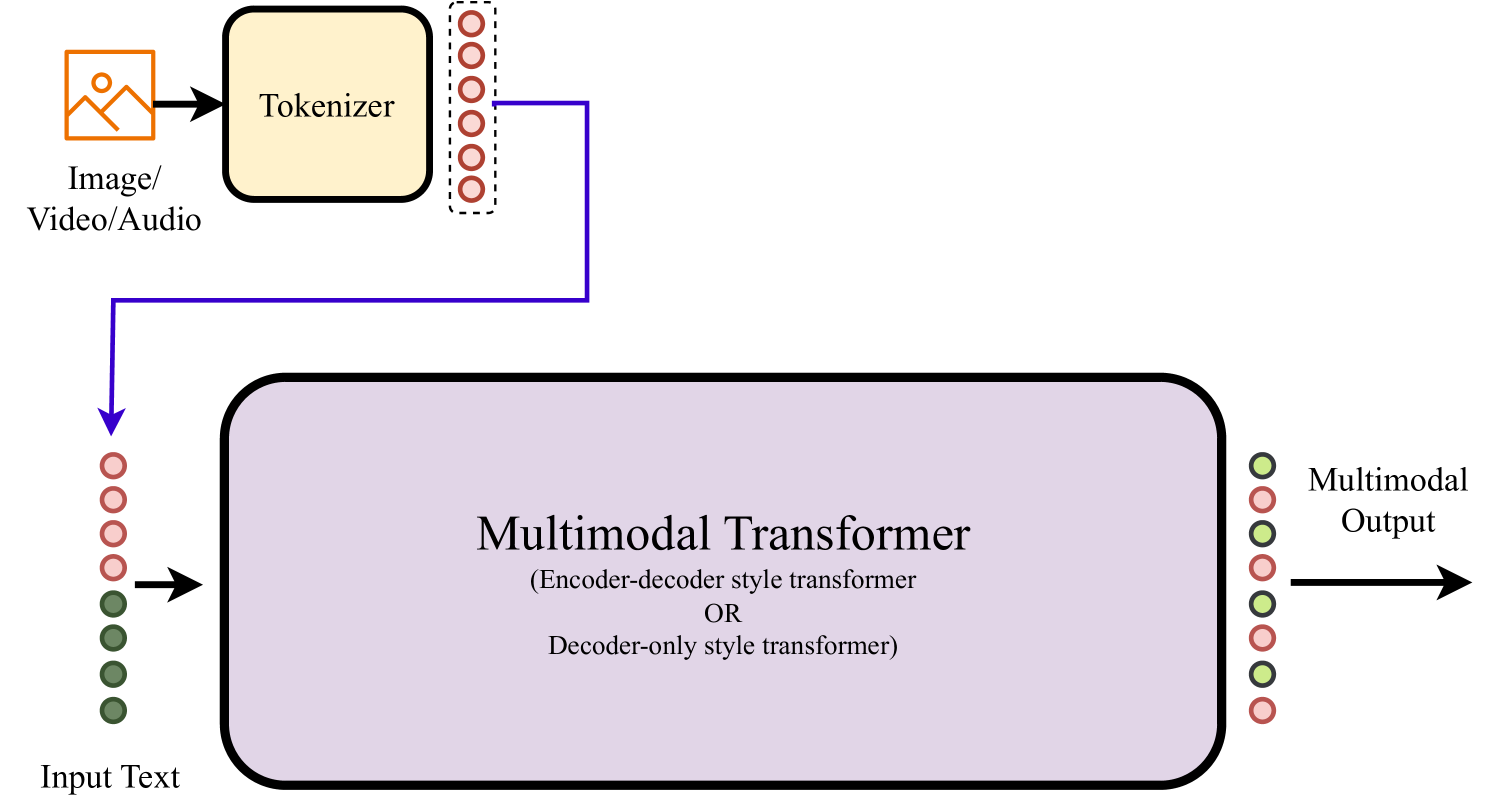
\includegraphics[width=0.9\linewidth]{Figures/fig_21.png}
    \caption{Example of multimodal transformer architecture}
    \label{fig:enter-label}
\end{figure}
This architecture in multimodal large language models is applied in order to do two main tasks:
\begin{enumerate}
    \item \textbf{Image-To-Text:} This task consists of assigning a textual description to an image by recognizing the elements present within it.


    \item \textbf{Text-To-Image:} This task consists in generating an image, given a text by recognizing the meaning and the semantics of the words.
\end{enumerate}
There are several multimodal large language models capable of solving these tasks, representing evolutions of large language models already introduced and described. The main MLLMs we will cover are the following:

\begin{itemize}
    \item \textbf{GPT-4}

    \item \textbf{Google Gemini} 

    \item \textbf{GLaMM}

    \item \textbf{BLIP-2}
\end{itemize}

\subsubsection{GPT-4}
GPT-4 is the latest version of the most popular large language model: GPT. Released in March 2023, it became available to premium users of the ChatGPT platform in three distinct versions: GPT-4, GPT-4 Turbo, and GPT-4o (omni). These versions represent an evolution of the GPT-3 model, enhancing performance, response speed, and processing a higher number of tokens per minute.\cite{insights_gpt4} The multimodal version of GPT-4, known as GPT-4o where the "o" stands for "omni," highlighting the "omniscience" of this model is capable of:
\begin{itemize}
    \item Real-time voice communication: GPT-4o is able to engage in real-time voice conversations, understanding spoken input and generating natural-sounding voice responses.

    \item Real-time vision: GPT-4o is able to process and understand vision data like images and video and their semantics. The model can generate an image starting from text and applying styles or generating descriptions of an image.

    \item Code Reading Through Vision: this feature is very useful for developers, given a screen of an IDE like Eclipse or Visual studio code. GPT-4o can read and understand the code inside the image, giving useful responses to developers.

    \item Data and Chart Reading: GPT-4o can read and interpret data in forms of charts and graphs, giving useful insights.
\end{itemize}
These features make GPT-4o a versatile and powerful tool applicable in many sectors, with particular emphasis on programming and data analysis. Details regarding the dataset, number of parameters, and training technique are not disclosed for competitive reasons.
\subsubsection{Google Gemini}
The latest evolution of Google's large language models is Gemini, this model has been introduced in 2023 and it is the evolution of Bard: the chatbot based on PaLM which I discussed in the previous section. Google Gemini, like GPT-4, is not only capable of generating and understanding text but can also interpret images, videos, and audio, accepting multimodal prompts.\cite{gemini_introduction}
Gemini has proven to be superior to its rival GPT-4 on various benchmarks, achieving results of up to 90\% accuracy.
\subsubsection{GLaMM}
GLaMM (Grounding LLM) is a multimodal large language model that integrates natural language with object segmentation masks in images, combining scene-level, region-level, and pixel-level understanding. 
The model uses an auto-encoder to process images and an LLM to understand natural language. The encoder is based on ViT-H/14 from CLIP and there are a grounding image encoder, a pixel decoder, and a region encoder inspired by GPT4Rol. The LLM is based on Vicuna with 7 billion parameters, and the vision-language and language-prompt projection layers are implemented using a 2-layer MLP activated with GELU. \cite{rasheed2024glamm}
\begin{figure}[H]
    \centering
    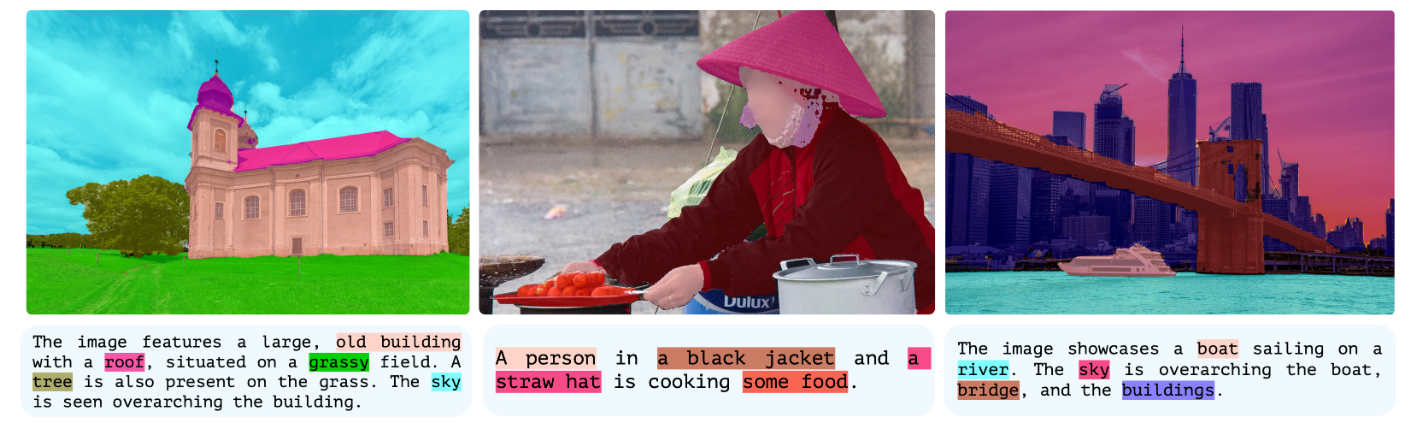
\includegraphics[width=0.9\linewidth]{Figures/fig_23.png}
    \caption{GLaMM object segmentation}
    \label{fig:enter-label}
\end{figure}
The source code is available on the official GitHub repository:\\ \href{https://github.com/mbzuai-oryx/groundingLMM}{https://github.com/mbzuai-oryx/groundingLMM}

\subsubsection{BLIP-2}
BLIP (Bootstrapping Language-Image Pre-training) is a multimodal large language model developed in 2023 by Salesforce: an IT company in the filed of CRMs.
The model has 188 millions of parameters and the architecture is composed by three principal components:
\begin{enumerate}
    \item Image encoder: There is a vision encoder ViT-L/14.

    \item Q-Former: The query transformer (Q-Former) matches the embedding representation of the image with the text.

    \item Large Language Model: The llm is based on T5 and gets the input from the Q-Former in order to create image descriptions.
\end{enumerate}
BLIP-2 architecture is designed to generate captions starting from images, this task is called vision-to-language generation. This task is performed in a zero-shot setting: the model has no similar example to the image. Another task that the model can perform is visual question answering (VQA), answering questions about image content on which it can reason about interpreting complex scenes and making inferences about them. 
\begin{figure}[H]
    \centering
    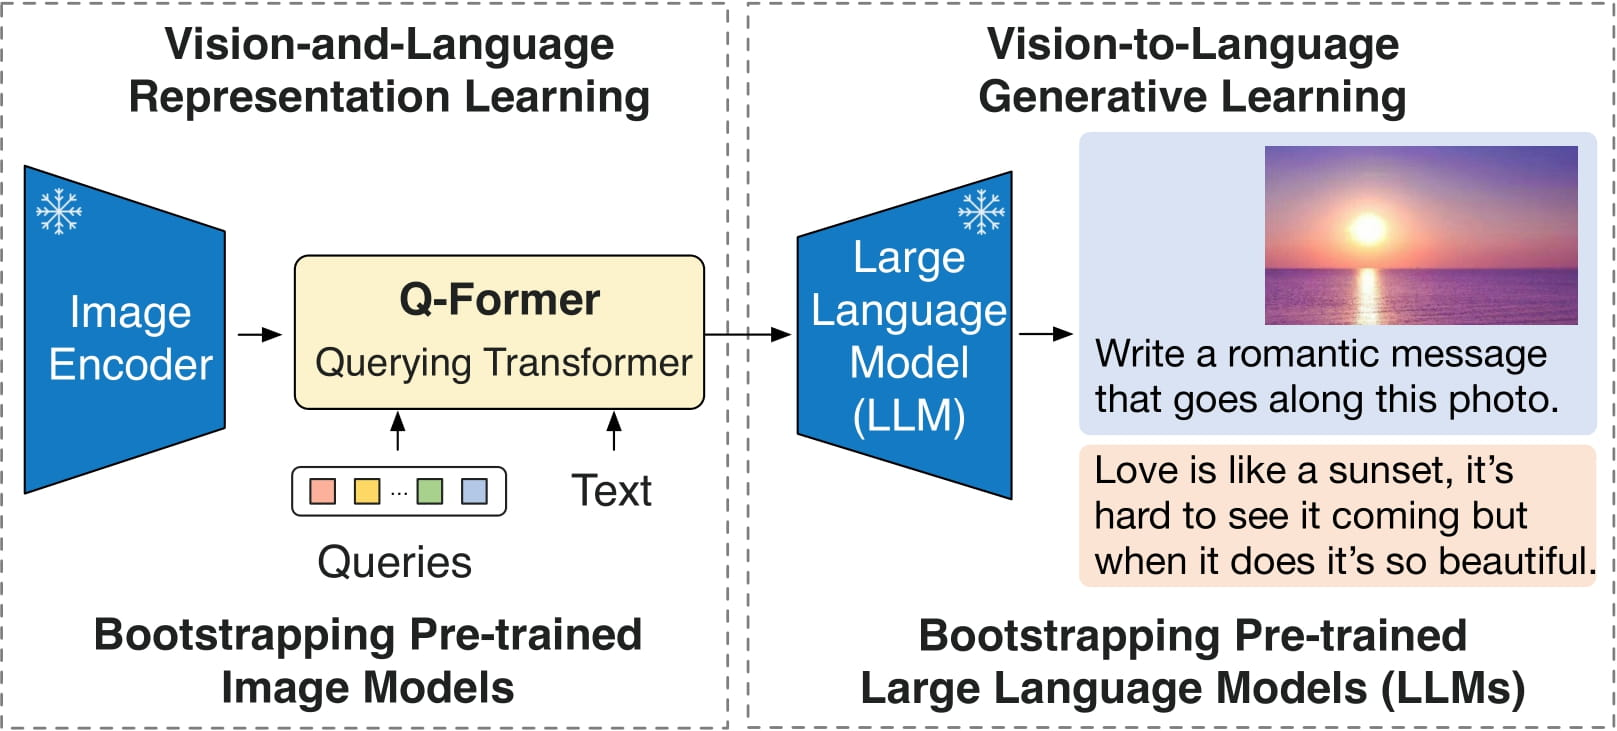
\includegraphics[width=0.7\linewidth]{Figures/fig_24.jpg}
    \caption{BLIP-2 architecture}
    \label{fig:enter-label}
\end{figure}
\newpage
\section{Prompt engineering}
\subsection{What is prompt engineering?}
At the core of interaction with large language models are prompts, a prompt is an instruction written in natural language given as input to a large language model to generate a response or action.\cite{llm_prompt}
A prompt can be written without a criteria or following specific prompting techniques that describe the structure, the application of those techniques iteratively is the prompt engineering\cite{schulhoff2024prompt}, in this process there is the modification of the structure in order to get better and more accurate results from the model. A prompt can be structured in different ways, the first way is writing the instructions and include a direct question like:
\begin{lstlisting}
How should I write my college admission essay? Give me suggestions about the different sections I
should include, what tone I should use, and what expressions I should avoid.   
\end{lstlisting}

The second way is just the specification of the input without any question like:
\begin{lstlisting}
Tell me five good books to read. 
\end{lstlisting}
In some cases it useful to provide context and examples in the prompt or specify the output formatting because basically the output is plain text for example:
\begin{lstlisting}
Tell me five good books to read.
Give me the list into a csv.
\end{lstlisting}
We can see a prompt like a mathematical function that takes in input a text and gives an output $ f(x) = y$ in which $f()$ is the template applied to the text of the problem, for example if we want to translate a phrase in english: 
\begin{lstlisting}
Translate {X} in english
\end{lstlisting}
This is just a simple technique in which there is the manual creation of the template but there are in literature more complex techniques that we are going to discuss.
\subsection{Prompt engineering techniques}
Prompt engineering techniques involve structuring a prompt in a specific way according to a particular strategy in order to obtain more accurate responses and a better understanding of the problem to be solved by the model. The first and simplest technique is the \textbf{Zero-shot prompting} in which no example is provided, and the large language model has no prior knowledge of the context, generating the output based solely on the given input prompt. An example is the following: 
\begin{lstlisting}
Classify the text into neutral, negative or positive. 
Text: I think the vacation is okay.
Sentiment:   
\end{lstlisting}
In \textbf{Few-shot prompting}, on the other hand, the input prompt provided to the large language model includes a few examples, with the aim of not only achieving a better understanding of the context (something that was not possible with zero-shot prompting) but also obtaining improved performance, as we can see in the following example:
\begin{lstlisting}
Task: Translate the following sentences from italian to english.

Example "Oggi il tempo e' bello" output: "The weather is nice today"

input: "Mi piace leggere libri" // output: I love reading books
\end{lstlisting}
The two techniques are thus based on a single prompt, but we can use multiple prompts, in the multi-prompt learning  
we can follow a reasoning process and in this sense the main technique is \textbf{Chain-of-Thought (CoT) Prompting}, where logical reasoning is done step by step to achieve more structured and accurate responses. An example is the following:
\begin{lstlisting}
Q: Roger has 5 tennis balls. He buys 2 more cans of tennis balls. Each can has 3 tennis balls. How many tennis balls does he have now? 
A: Roger started with 5 balls. 2 cans of 3 tennis balls each is 6 tennis balls. 5 + 6 = 11. The answer is 11.  
Q: The cafeteria had 23 apples. If they used 20 to make lunch and bought 6 more, how many apples do they have?

Model output: The cafeteria had 23 apples originally. They used 20 to make lunch. So they had 23 -  20 = 3.  They bought 6 more apples, so they have 3 + 6 = 9. The answer is 9.   
\end{lstlisting}
The main issue with this technique is the manual intervention required, as the user must manually provide the reasoning that the large language model will follow. To address this problem, a variant called \textbf{Automatic Chain-of-Thought (Auto-CoT) Prompting} was introduced. Instead of manually providing the reasoning chain, the prompt includes a simple phrase, "Let's think step-by-step," to automatically generate multiple reasoning chains.\\
Both CoT and Auto-CoT follow a single reasoning path but we can generate multiple reasoning paths and choose the best answer, this is the basis of the \textbf{Self-consistency prompting}\cite{wang2022self}. Multiple reasoning paths are created using chain of thought prompting and then evaluating responses.\\
Another technique that generate mutliple resoning paths is the \textbf{Thread of Thought (ThoT)}
prompting technique. In practice, a tree-of-thought is automatically generated, and each step of the reasoning process is evaluated automatically. Additionally, by combining graph search algorithms such as BFS (Breadth-First Search) and DFS (Depth-First Search), the ability to evaluate different reasoning paths is improved.
\begin{figure}[H]
    \centering
    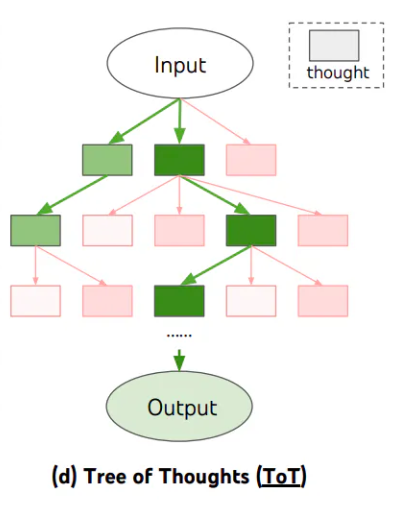
\includegraphics[width=0.4\linewidth, height=7cm]{Figures/fig_6.png}
    \caption{Thread of Thought (ThoT) Prompting}
    \label{fig:enter-label}
\end{figure}
It is possible to adapt the large language model to the different reasoning task using the \textbf{Active prompting} that enhances performance introducing a mechanism for determining the most impactful questions for annotation. Starting from a set of questions $Q = \{q_1, q_2, ..., q_n\}$ the goal is to annotate the answers ($a_i$) obtained with intermediate steps ($c_i$):\\ $E = \{(q_1, c_1, a_1), (q_2, c_2, a_2) ..., (q_n, c_n, a_n)\}$ there is the measurement of the disagreement of the answers, the entropy and the variance. Once the best k-questions with their respective answers are selected, self-consistency is applied (a technique that generates multiple outputs from a single prompt) \cite{wang2022self}, and finally, the most relevant answers are chosen.\\
Those technique involving multiple prompts are useful in order to decide the best reasoning strategy but we can also decide not to use any complex reasoning but a more simple strategy that can involve the ensembling, the augmentation, the composition or the decomposition of a single prompt.\cite{liu2023pre} In \textbf{prompt ensembling} there is the combination of different prompt on the same subject to get the response for example:
\begin{lstlisting}
PR1: China's capital is [X]
PR2: [X] is capital of China
PR3: The capital of China is [X]
\end{lstlisting}
To choose the response, we can apply several strategies, including majority voting, weighted voting ecc.. 
In \textbf{prompt augmentation} there are additional examples providing the model an example of response (this is similar to few-shot prompting) for example:
\begin{lstlisting}
Main prompt: 6 + 8 = [X]
PR1: 1 + 1 = 2
PR2: 2 + 5 = 7
\end{lstlisting}
In \textbf{prompt composition} there is a composition of two or more subprompts in order to get the final prompt in contrast in \textbf{prompt decomposition} one main prompt is decomposed in two or more smaller subprompts.
In large language models, there is a significant issue that leads to incorrect responses, known as the problem of hallucinations. We refer to hallucination, in the context of LLMs, when there is the generation of texts or responses that are grammatically and syntactically correct but deviate from the given inputs or do not align with factual accuracy. \cite{ye2023cognitive} Prompt engineering techniques can help reduce this phenomenon,the main technique is \textbf{Retrieval Augmented Generation (RAG)}. In this approach, starting from an input, a knowledge base of sources (web pages, articles, etc.) is created, and the text from these sources is incorporated into the subsequent input, providing context and generating more accurate and reliable responses. Another technique, that combines reasoning and acting with LLMs, is the \textbf{ReAct Prompting}. A ReAct prompt consists of few-shot task-solving trajectories, with human-written text reasoning traces and actions, as well as environment observations in response to actions \cite{react_llm} an example, provided by the authors is the following: 
\begin{figure}[H]
    \centering
    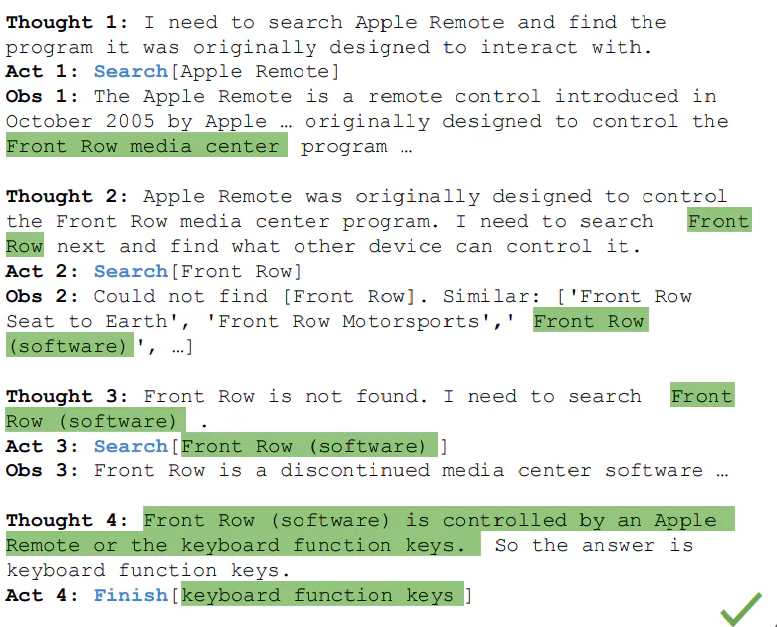
\includegraphics[width=0.7\linewidth]{Figures/fig_7.png}
    \caption{ReAct Prompting}
    \label{fig:enter-label}
\end{figure}
The improvement in performance and accuracy of the responses obtained from the large language model can also be achieved by incorporating the user's emotions into the prompt, known as \textbf{Emotion Prompting}.
Incorporating emotions can be useful in tasks such as sentiment analysis of a sentence, but this is not the case for code generation, for which various prompt engineering techniques have been introduced. \\
An evolution of the previously described Chain-of-Thoughts is \textbf{Program of Thoughts (PoT) Prompting} \cite{chen2022program}, where the large language model is given a prompt containing intermediate steps that include mathematical expressions or source code, as we can see in the following figure:
\begin{figure}[H]
    \centering
    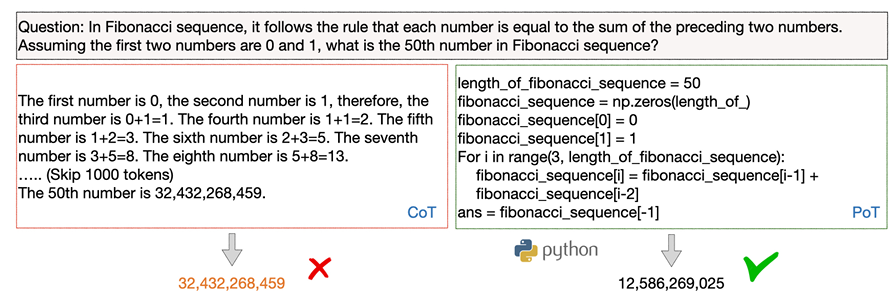
\includegraphics[width=0.7\linewidth]{Figures/fig_8.png}
    \caption{Program of Thoughts (PoT) Prompting}
    \label{fig:enter-label}
\end{figure}
Another approach is the \textbf{Scratchpad Prompting} in which there is the generation of an arbitrary sequence of intermediate tokens before providing the final answer. The sequence is given in a tag called "scratch"\cite{scratch}\cite{nye2021show} in which the user writes intermediate steps useful to the large language model as shown below: 
\begin{lstlisting}
<scratch>
2 9 + 5 7 ,  C: 0
2 + 5 , 6 C: 1    # added 9 + 7 = 6 carry 1
, 8 6 C: 0        # added 2 + 5 + 1 = 8 carry 0
0 8 6
</scratch>
8 6
\end{lstlisting}
In the example above we teach the LLM the addition of two numbers. \\
The techniques illustrated aim to reduce calculation and output generation errors produced by large language models through examples or reasoning sequences provided manually. The \textbf{Rephrase and Respond (RaR) Prompting}\cite{deng2023rephrase} technique automatically allows for the correction and improvement of the LLM's response through the prompt:
\begin{lstlisting}
"{question}" Rephrase and expand the question, and respond.
\end{lstlisting}
This approach has four main advantages:
\begin{enumerate}
    \item It lets the LLM self-improve the prompts while maintaining the context of the original query.

    \item It allows better aligning the human’s intended query with LLM’s preferred style of question.

    \item It expands the LLM’s thought process and adding a step that will not naturally appear when using CoT.

    \item It provides an approach for humans to interpret how LLMs understand the questions.
\end{enumerate}
Another technique to obtain more accurate and comprehensive responses is the \textbf{Take a Step Back Prompting}\cite{zheng2023take}, which consists of two steps. The first step involves inputting a specific question, and subsequently (step-back) inputting a more abstract, high-level question related to the task, as shown in the following figure:
\begin{figure}[H]
    \centering
    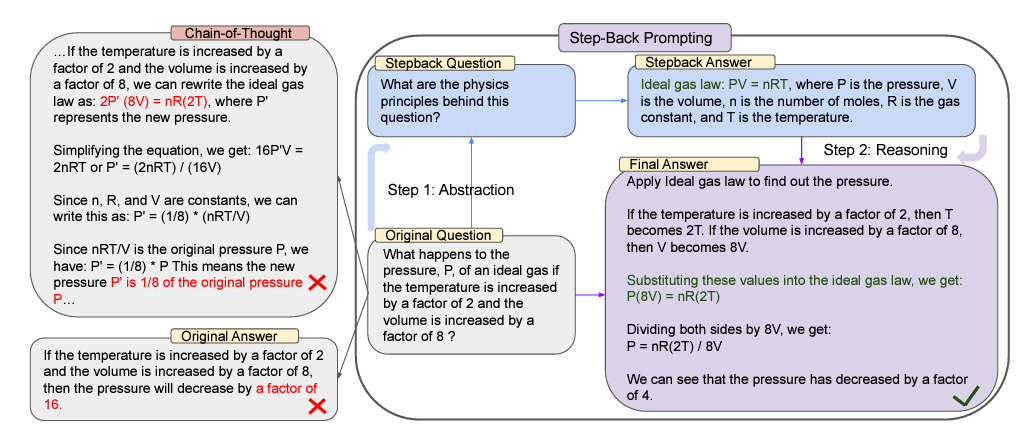
\includegraphics[width=0.9\linewidth]{Figures/fig_9.png}
    \caption{Take a Step Back Prompting}
    \label{fig:enter-label}
\end{figure}

\subsection{Prompt engineering in multimodal LLMs}
State-of-the-art prompt engineering techniques aim, when given as input to a large language model, to generate text. The most recent advancements in technology allow for incorporating images into the prompt or generating images using multimodal large language models. 
Main tasks involving multimodal large language models are:
\begin{itemize}
    \item Image generation
    \item Image classification
    \item Image editing
    \item Image classification
\end{itemize}


A preliminary approach to image classification is the use of two techniques, namely zero-shot prompting and few-shot prompting. \cite{chen2023unleashing} In zero-shot prompting for image generation, no input examples are provided, but only the instruction to be executed, for example:
\begin{lstlisting}
Classify the follwing image: [image.png]
\end{lstlisting}
In few-shot prompting examples are provided to the model, for example:
\begin{lstlisting}
Given: [image1.png], [image2.png], [image3.png], classify the following image: [image.png]
\end{lstlisting}
Zero-shot prompting and few-shot prompting can be also used in image generation, this task is more complex and it can be useful to incorporate user feedback that helps improve the generated image. An example is drawing a stick figure using letters of the alphabet \cite{proptingguide_image}, where the process starts from an initial prompt, such as:
\begin{lstlisting}
Produce TikZ code that draws a person composed from letters in the alphabet. The arms and torso can be the letter Y, the face can be the letter O (add some facial features) and the legs can be the legs of the letter H. Feel free to add other features.    
\end{lstlisting}
The generated image is refined by adding details: 
\begin{lstlisting}
- The torso is a bit too long, the arms are too short 
  and it looks like the right arm is carrying the face instead of the face being right above the torso. Could you correct this please? 

- Please add a shirt and pants.
\end{lstlisting}
As we can see in the following example, where the latest version of ChatGPT, GPT4, has been applied:
\begin{figure}[H]
    \centering
    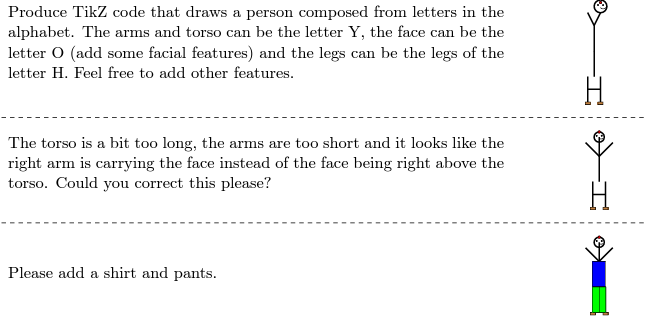
\includegraphics[width=0.8\linewidth]{Figures/fig_10.png}
    \caption{Drawing using GPT4}
\end{figure}
In image generation the characteristics of an image can be specified not only using user feedback but also using \textbf{style modifiers}. Style modifiers are  descriptors that consistently produce certain styles, for example: "tinted red", "made of glass", and combining those together they produce a more specific style. \cite{lp_style} 
For example we want to generate using DALL-E a picture of a pyramid, the first picture is generated without using any modifier:
\begin{figure}[H]
    \centering
    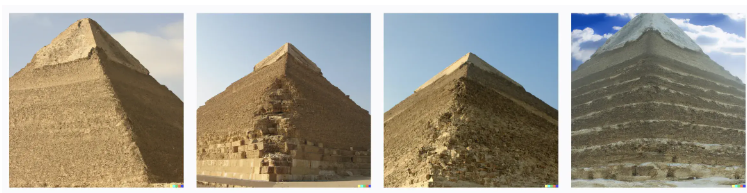
\includegraphics[width=0.9\linewidth]{Figures/fig_11.png}
    \caption{Pyramid picture with no modifiers}
    \label{fig:enter-label}
\end{figure}
The second picture is generated using the prompt with three modifiers: \textit{A pyramid made of glass, rendered in Unity and tinted red} getting the following result:
\begin{figure}[H]
    \centering
    
\includegraphics[width=0.9\linewidth]{Figures/fig_12.png}
    \caption{Pyramid picture with modifiers}
    \label{fig:enter-label}
\end{figure}
In the prompt, in order to improve quality, we can add generic adjectives like: \textit{"amazing"}, \textit{"good"}, \textit{"beautiful"} that are called \textbf{quality boosters}. \cite{oppenlaender2023taxonomy} 
The Latin motto \textit{"repetita iuvant"} that means that repeating words is useful can be applied in a certain sense in a prompt for image generation. In the \textbf{repetition technique} if we want to give more importance to some adjective instead of another it is possible to repeat more times the word, giving to it emphasis. For example if we want to generate an image of a waterfall for example but we want to emphasise the beauty of the picture we can use this following prompt:
\begin{lstlisting}
A very very very very very beautiful painting of a mountain next to a waterfall
\end{lstlisting}
In this case the word "very" is repeated five times in order to give more importance to the adjective beautiful.\\
Repeating terms in a prompt can be weird and inaccurate, it is possible to use \textbf{weighted terms technique}\cite{weighted_terms} in which a term has a numerical value (positive or negative) that corresponds to the weight, the importance of that term. For example if we want to generate a picture of a mountain without trees, we use this prompt:
\begin{lstlisting}
mountain | tree:-10.
\end{lstlisting}
in which the tree has negative weight and it doesn't have importance getting this result:
\begin{figure}[H]
    \centering
    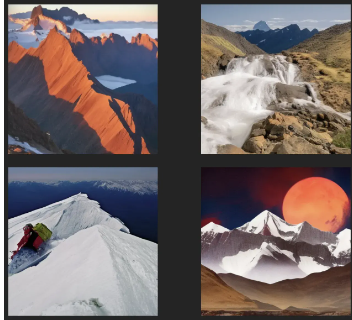
\includegraphics[width=0.5\linewidth]{Figures/fig_15.png}
    \caption{Weighted terms image}
    \label{fig:enter-label}
\end{figure}

Another approach in image generation is negative prompting, negative prompts allow users to exclude unwanted features and enhance the quality output.
Negative prompts are complementary to  positive prompts which describe what the user wants, including the main subject and how it should look.\cite{medium_negative}
For example, we want to generate using a diffusion model a portrait of a man without mustache so the prompt is:
\begin{lstlisting}
- Positive prompt: Portrait photo of a man.
- Negative prompt: Mustache
\end{lstlisting}
Negative prompts can be applied on any image feature like: colors, lighting problems, unwanted elements, image quality and style.\\
Multimodal large language models can be used not only to generate photorealistic images but also artistic images following the style of a particular artist or artistic movement, as discussed in the paper \textit{Design Guidelines for Prompt Engineering Text-to-Image Generative Models} \cite{liu2022design}. The study using the CLIP model generates images in 51 artistic style using the following prompt:
\begin{lstlisting}
SUBJECT in the style of STYLE
\end{lstlisting}
and its permutations like:
\begin{itemize}
    \item A MEDIUM of SUBJECT in the STYLE style - a painting of love in the abstract style

    \item A STYLE MEDIUM of a SUBJECT - an abstract painting of love

    \item SUBJECT STYLE - love abstract art

    \item SUBJECT.STYLE - love.abstract art

    \item SUBJECT in the STYLE style - love painted in the abstract art style

    \item SUBJECT VERB in the STYLE style - love painted in the abstract style

    \item SUBJECT made/done/verb in the STYLE art style - love done in the abstract art style

    \item SUBJECT with a STYLE style - love with an abstract art style
\end{itemize}
A total of 1,296 were generated with 144 permutations for each of the 9 selected subjects: love, hate, happiness, sadness, man, woman, tree, river and dog. The applied prompting technique has produced interesting results that can be qualitatively evaluated and still reflect the desired styles provided as input in the prompt.\\
In the techniques previously described, the prompt consists only of text, but in some models, it is possible to integrate one or more images along with the text, not only to generate images but also to obtain responses related to input images. The \textbf{Multimodal Chain-of-Thought} prompting technique\cite{zhang2023multimodal} is a variation of the Chain-of-Thought technique (CoT), this technique in Multi-CoT is enhanced by incorporating in the prompt text and visual inputs. The technique consists in two stages:
\begin{enumerate}
    \item Rationale generation: the model processes the multimodal inputs in order to generate an intermediate reasoning chain (rationale). The rationale explains the logical steps required to arrive at the final answer, using both textual and visual content as context.

    \item Answer inference: the generate rationale is combined with the original input and used by the model to infer the final answer.
\end{enumerate}
as we can see in the figure below:
\begin{figure}[H]
    \centering
    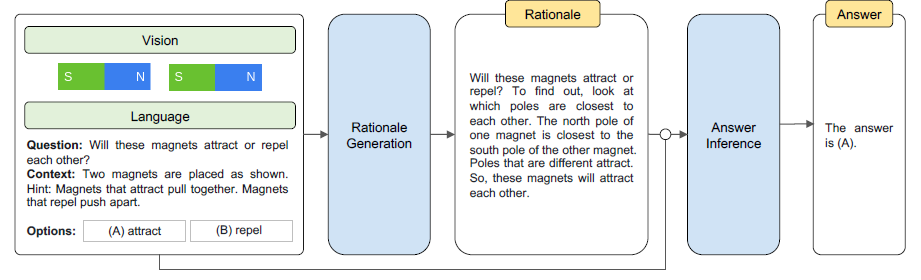
\includegraphics[width=0.9\linewidth]{Figures/fig_16.png}
    \caption{Multimodal Chain-of-Thought}
    \label{fig:enter-label}
\end{figure}
The technique has been tested on T5, UnifiedQA and FLAN-Alpaca and it has a good accuracy averaging around 85\%.\\
Similar to the multimodal chain-of-thought, the \textbf{Chain of Images (CoI)} prompting technique \cite{meng2023chain} generates a series of images as intermediate representations in order to solve problems starting from a textual prompt. Although the technique is innovative as it uses images instead of text, it is not applicable to large language models outside the SyMLLM framework, which is capable of reasoning using this technique. \\\\